% INPUT FILE FOR NUCLEAR ENGINEERING RESEARCH GROUPS AND STUDENTS 
% ------------------------------------------------------------ 
% Each research group has a page here describing their work and student members.
% This page begins with a `\grouptitle` marker specifying the group's name.
% Next follows the description, which is currently free-formatted. You might need to do this yourself.
% Then follows the student members; each student gets a tile. (Formatting for this tile is defined in the preamble.)
% Each student tile is then included in a row of two tiles. (Its formatting is also defined in the preamble.)
% The sytax is as follows:
% \studentrow{
%		\studenttile{image_name_student1}
%		{Name student 1}
%		{Position student 1}
%		{Email student 1}
%		{Description student1}
%	}{
%		\studenttile{image_name_student2}
%		{Name student 2}
%		{Position student 2}
%		{Email student 2}
%		{Description student2}
%}
% NOTE: The first student row includes the "Members" header, and so must be indicated with the `\firststudentrow` command, instead of the `\studentrow` command (all arguments are otherwise the same).

\newgeometry{margin=2cm}
\addcontentsline{toc}{section}{Research Groups}
\section*{Research Groups}

\grouptitle{BioActinide Chemistry}

\begin{minipage}{0.7\textwidth}
	The multidisciplinary research undergone in the group is at the interface of coordination chemistry, analytical chemistry, photophysics, biological chemistry, health physics, pharmacology, and molecular and cellular biology. 
	We study the effects of heavy element exposure and contamination on different biological systems in addition to the coordination chemistry and metabolic properties of lanthanide and actinide complexes formed with synthetic and biological ligands. 
	Our goals are to gain a better understanding of the biological coordination chemistry and toxicity mechanisms of the f-elements and to develop specific strategies for decontamination, remediation, and separation. 
	Other applications include the development of new antimicrobial strategies that target metal acquisition systems, PET imaging systems, and the design of advanced alpha-immuno therapeutic and diagnostic agents. 
	A new addition to the Nuclear Engineering department as of January 2018, the BioActinide Chemistry group is housed partially on campus and partially at LBNL, where we work closely with the Nuclear Sciences Division. 
	As of February 2019, the group includes 4 graduate students, 7 postdocs, 9 undergraduates,1 staff scientist, and a partridge in a pear tree.
\end{minipage}
\begin{minipage}{0.3\textwidth}
	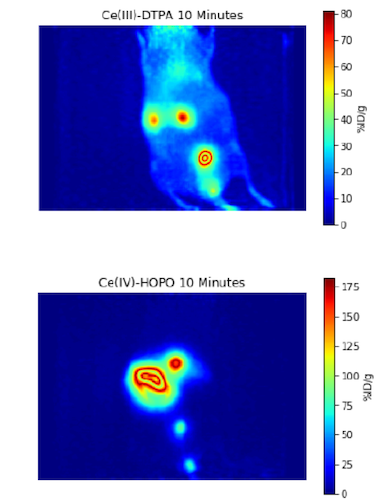
\includegraphics[width=\textwidth]{research_groups/bioactinide_chemistry/mouse_pet}
\end{minipage}

\vspace{0.5cm}
\begin{minipage}{0.40\textwidth}
	\begin{center}
		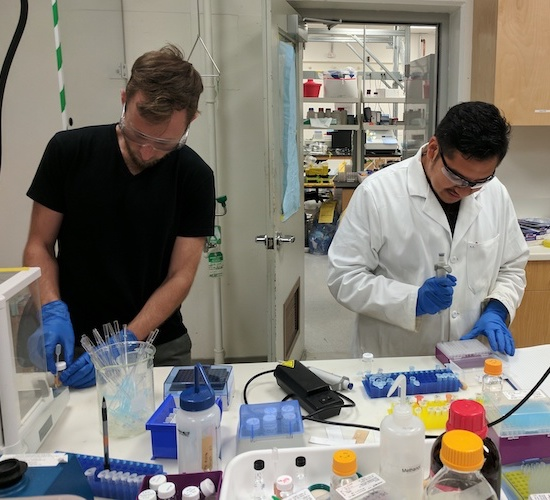
\includegraphics[height=175px]{research_groups/bioactinide_chemistry/korey-abel_labwork}
	\end{center}
\end{minipage}
\begin{minipage}{0.33\textwidth}
	\begin{center}
		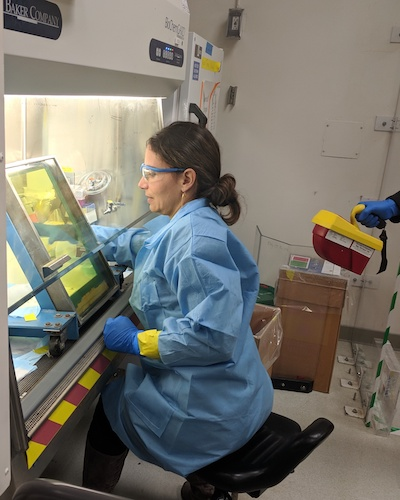
\includegraphics[height=175px]{research_groups/bioactinide_chemistry/rebecca_134Ce}
	\end{center}
\end{minipage}
\begin{minipage}{0.17\textwidth}
	\begin{center}
		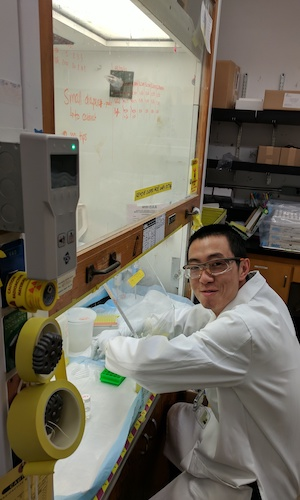
\includegraphics[height=175px]{research_groups/bioactinide_chemistry/yufei_hood}
	\end{center}
\end{minipage}

\firststudentrow{
	\studenttile
	{students/tyler_bailey}
	{Tyler Bailey}
	{}
	{tybtab@berkeley.edu}
	{Tyler is a bionuclear physicist that is working on the development and characterization of surrogate, positron-emitting complexes for Targeted Alpha Therapy. He loves dogs, guinea pigs, tortoises, video games, books, radiation, and movies.}
}{
	\studenttile
	{students/kathy_shield}
	{Kathy Shield}
	{}
	{kshield@berkeley.edu}
	{Kathy is working on solution thermodynamics characterization of actinium complexes, with the goal of identifying better ligands for medical isotope complexation and cancer therapeutics applications.
	She worked at Los Alamos National Lab in the summer of 2017 on silicon drift detectors and can attest that the summers are colder here than in New Mexico, while winters are colder in Boston than Berkeley. 
	When not in class or at the lab, you can find her skiing, dancing, reading, or hiking.}
}

\studentrow{
	\studenttile
	{students/yufei_wang}
	{Yufei (Albert) Wang}
	{}
	{ywang16@berkeley.edu}
	{Albert is a PhD student working on the aqueous reprocessing of used nuclear fuels, specifically on the separation of lanthanides and actinides. He used to study at Tsinghua University and the University of Tokyo before he came to the US, so he's trilingual. Other than learning diverse cultures through studying abroad he is also interested in sports, such as badminton, swimming, hiking, and skiing.}
}{}

\grouptitle{Applied Nuclear Physics and Radiation Detection}

Our radiation detection and measurement research group at UC-Berkeley comprises two main groups: the BeARING (Berkeley applied Research for the Imaging of Neutrons and Gamma-rays) on campus, and the Applied Nuclear Physics (ANP) group at Lawrence Berkeley National Lab (LBL). 
Additionally, several members of the BeARING group are involved in graduate research at other facilities, including Lawrence Livermore National Lab (LLNL) and Sandia National Lab. 
The research undertaken by members of the group span nearly the entire spectrum of radiation detection and measurement (pun intended). 
On the technology side, the semiconductor fabrication laboratory is involved in projects for the development of novel semiconductor detectors and detector readout methods. 
The high-energy and spatial resolution of these novel systems are tightly coupled to gamma-ray imaging applications in astrophysics, biomedical imaging, and nuclear safeguards/nonproliferation.

In an effort to demonstrate the breadth of research undertaken by the BeARING group, several active projects are detailed below.

\textbf{Algorithm development}\\
Developing innovative algorithms and frameworks to enable more robust radiation detection capabilities, such as modeling variable gamma-ray backgrounds, deploying spectroscopic detection algorithms, and attempting real-time, 3-D gamma-ray image reconstruction.

\textbf{Contextual Sensor and Radiation Data Fusion}\\
Fusing contextual and radiation data enables the visualization of radioactive sources and contamination. 
This capability has been applied to a variety of platforms (drones, cars, SUVs, helicopters) for applications including environmental mapping and decommissioning in Fukushima Prefecture.
 
\textbf{Data management}\\
Developing web-based platforms for data exploration, retrieval, on/offline analysis, and sharing between DOE labs and contractors.
Examples include the Berkeley Data Cloud, which disseminates data for initiatives like the Multiple Informatics for Nuclear Operations Scenarios (MINOS) Venture. 

\textbf{Detector development (Semiconductor Detector Laboratory)}\\
Pushing the limits of ultra-low noise and high-rate Germanium detectors, enabling next generation gamma-ray detection for nuclear structure physics, neutrino and dark matter science, and astrophysics. 
 
\textbf{Sensor networks}\\
Creating large-scale, ubiquitous, and distributed radiation detection sensor networks to passively detect, localize, and track radiological and/or nuclear threats.

\firststudentrow{
	\studenttile
	{students/grey_batie}
	{Grey Batie}
	{he/him/his; they/them/theirs}
	{batie@berkeley.edu}
	{Grey's current research focuses on developing unique methods to design and operate reprocessing facilities and other nuclear material bulk handling facilities, to enable the detection of inadvertent or deliberate hold up of fissionable material. 
	Grey earned a B.S. in both Nuclear Engineering and in Physics from MIT, and a M.S. in Medical Physics from the University of Wisconsin Madison. 
	Their interests include recruitment, retention, and advocacy for minority students in the sciences.}
}{
\studenttile
	{students/justin_ellin}
	{Justin Ellin}
	{}
	{jrellin@berkeley.edu}
	{Justin is a Nuclear Engineering graduate student at the University of California, Berkeley and a NSF research fellow. 
	He is interested in the study of high-energy gamma ray imaging systems for high radiation field environments. 
	He has a B.A. in Physics from UC Berkeley and worked for several years in the Physics Research Laboratory at UCSF. 
	His interests include science education for under-represented high school students and public outreach about our radioactive world.}
}

\studentrow{
	\studenttile
	{students/emily_frame}
	{Emily Frame}
	{}
	{eaframe@berkeley.edu}
	{Emily's current research is on developing a static detection system that incorporates a 4pi visual camera for tracking of nuclear material. 
	Emily received her B.S. in Nuclear Engineering at UT Knoxville and then spent two years as an English lecturer and researcher in the Department of Nuclear Reactors at the Czech Technical University in Prague. 
	Outside of research, Emily’s interests include swimming and playing Hungarian mafia.}
}{
\studenttile
	{students/adam_glick}
	{Adam Glick}
	{}
	{adam\_glick@berkeley.edu}
	{Adam is working on neutron imaging using a neutron scatter camera to determine the energy and fluence of neutrons produced during particle cancer therapy. 
	He is also interested in improving the Monte Carlo system, TOPAS, to better model radiation cancer therapy in clinical settings. 
	His outside interests include whiskey distillation to make craft whiskeys, going hiking around the Berkley hills, and running Spartan Races with his wife.}
}

\studentrow{
	\studenttile
	{students/rebecca_krentz-wee}
	{Rebecca Krentz-Wee}
	{}
	{rkw@berkeley.edu}
	{Rebecca researches radiation detection using coded aperture imaging and applications in arms control treaty verification. 
	She likes board games, cryptic crosswords, and exploring the Bay Area.}
}{
	\studenttile
	{students/matt_marshall}
	{Matt Marshall}
	{}
	{mattmar2410@berkeley.edu}
	{Matt is a PhD student focusing on improving detection and localization of radiation on mobile detector systems. 
	Matt enjoys exploring different coffee shops, traveling, reading, and is also in pursuit of finding the best pizza place in the Bay Area!}
}

\studentrow{
	\studenttile
	{students/darrell_stepter}
	{Darrell Stepter}
	{}
	{darrell.stepter@berkeley.edu}
	{A major in US Army, Darrell researches the effects of gamma attenuation on radioactive source detection/localization in urban areas}
}{
	\studenttile
	{students/yifan_zheng}
	{Yifan Zheng}
	{}
	{yifanzheng@berkeley.edu}
	{Yifan studies nuclear medicine imaging, in partnership with UCSF.}
}
\newpage

\grouptitle{Materials}

Our group applies experimental materials science techniques to understanding the effects of extreme environments as they are found in nuclear applications on structural materials. 
Our main points of research are:
\begin{itemize}
	\item Corrosion in liquid metals and other extreme corrosive environments.
	\item Small scale mechanical testing on materials for nuclear applications.
	\item Investigation and development of new alloying concepts.
\end{itemize}

\firststudentrow{
	\studenttile
	{students/tim_genda}
	{Tim Genda}
	{}
	{timothy\_genda@berkeley.edu}
	{Tim studies nuclear fireball chemistry, and enjoys hiking, skiing, nature, and photography.}
}{
	\studenttile
	{students/joey_kabel}
	{Joey Kabel}
	{}
	{joey.kabel@berkeley.edu}
	{Joey is currently researching the micro- mechanical properties of irradiated SiC/SiC composites for advanced reactor applications; applying SEM, FIB, Xray tomography, nano- indentation, and in situ testing techniques for material characterization. 
	Joey graduated from Washington State University in May 2015 with a B.S. in Materials Science and Engineering. 
	Outside of research he spends time participating in nuclear outreach, snowboarding, and happy hours.}
}

\studentrow{
	\studenttile
	{students/bill_mason}
	{Bill Mason}
	{}
	{masonw@berkeley.edu}
	{Bill is investigating high temperature geologic samples using femtosecond laser ablation ICP-MS. 
	His interests include mountaineering, motorcycles, sailing, and cave diving.}
}{
	\studenttile
	{students/franziska_schmidt}
	{Franziska Schmidt}
	{}
	{franziska\_schmidt@berkeley.edu}
	{Franziska is researching the corrosion of materials in a molten salt environment. 
	In her free time, Franziska enjoys happy hours, climbing, traveling, and losing money at the stock market.}
}

\studentrow{
	\studenttile
	{students/sarah_stevenson}
	{Sarah Stevenson}
	{}
	{srstevenson@berkeley.edu}
	{Sarah has a B.S. in Mechanical Engineering and previous experience as a Reactor Operator and Senior Reactor Operator, and developing miniature fission chambers with the Idaho National Laboratory (INL) and French Alternative Energies and Atomic Energy Commission (CEA). 
	Currently, she serves as a Physicist/Nuclear Engineer in the U.S. Air Force. 
	For her Ph.D., she's investigating the mechanical properties of deep-ion implanted materials. Sarah is a foodie and enjoys traveling and being active. }
}{
	\studenttile
	{students/evan_still}
	{Evan Still}
	{}
	{evanstill@berkeley.edu}
	{While at Berkeley, Evan partakes in swing dancing, blacksmithing, cooking, data mining, etc. 
	In his free time he looks at different ways to identify precipitates in steel.}
}

\studentrow{
	\studenttile
	{students/hi_vo}
	{Hi Vo}
	{}
	{sfhivo@berkeley.edu}
	{Hi researches in metal deformation and constitutive modelling. When he's not in the lab, Hi loves to travel and photograph landscapes.}
}{}

\grouptitle{Nuclear Waste Management}

Our group develops methods and models to study various aspects of nuclear fuel cycles and waste management. 
We use these tools to evaluate environmental impacts, management strategies, economics, and proliferation resistance of nuclear fuel cycles. 
At the moment, we have two ongoing projects:
\begin{enumerate}
	\item \textbf{Evaluation and design of nuclear waste containers for Fukushima fuel debris.}
	Management and disposal of the fuel debris created in the meltdowns at the Fukushima Daiichi nuclear power plant present unique challenges due to the random size and shape of the fuel particles and the relatively high enrichment of the heavy metal.
	We develop neutronics models to study the dose rates emitted from different types of waste canisters and evaluate margins protecting against recriticality of the fuel debris.
	\item \textbf{Methodologies for the evaluation of waste management strategies and applications to advanced nuclear fuel cycles.}
	Most fuel cycle analyses utilize insufficient metrics, such as waste mass and radiotoxicity, to quantify benefits in waste management. 
	These quantities are intrinsic properties of the waste streams but do not reflect management or disposal performance. 
	To that end, we develop more representative models that can be used to compare fuel cycles based on the management of their wastes. 
	Examples of these models include long-lived fission product inventory, repository footprint, and criticality safety.
\end{enumerate}

\firststudentrow{
	\studenttile
	{students/milos_atz}
	{Milos Atz}
	{}
	{milos.atz@berkeley.edu}
	{Milos is a PhD student studying the nuclear fuel cycle and waste disposal. In his spare time, he enjoys weightlifting, eating, hiking, and skiing.}
}{
	\studenttile
	{students/kyoungjin_lee}
	{Kyoungjin Lee}
	{}
	{kyoungjin\_lee@berkeley.edu}
	{Kyoungjin researches the retrieval of fuel debris from Fukushima Daiichi nuclear reactor. 
	He focuses on neutronic analysis of radiation dose and criticality safety of damaged nuclear fuels.}
}
\newpage

\hrulefill
\vspace{0.5cm}

{\huge Reactor Design and Neutronics}

The thrust of our research efforts into advanced reactor fuel cycles is the conception, design and analysis of advanced (Generation-IV+) nuclear reactors and nuclear fuel cycles. 
Specifically, the group has researched four innovative nuclear energy systems.
\begin{enumerate}
	\item Liquid-Salt cooled Advanced High Temperature Reactors (LS-AHTR also referred to as FHR for Fluoride cooled High temperature Reactors);
	\item Breed-and-Burn (B\&B) liquid metal cooled fast reactors,
	\item Fuel-self-sustaining thorium-fueled Boiling Water Reactors (BWR) and
	\item Molten-salt breeder and converter reactors (MSBR).
\end{enumerate}
In researching these systems, the role of the neutronics group is to develop both accurate and efficient core simulation software.
These tools can then be used to search for optimal core, reflector and control system designs. 
To validate results, the neutronics group frequently collaborates with others in the department (for example the thermal hydraulics group, the leader in FHR research) and internationally.

\firststudentrow{
	\studenttile
	{students/chris_keckler}
	{Chris Keckler}
	{}
	{keckler@berkeley.edu}
	{Chris works on safety and design aspects of sodium-cooled breed-and-burn fast reactors. 
	After moving from the flattest state in the country to California, he now loves biking down hills, but he hates biking up them.}
}{
\studenttile
	{students/dan_shen}
	{Dan Shen}
	{}
	{danshen.echo@berkeley.edu}
	{Dan comes from Tsinghua University in China. 
	Her past research is related to sensitivity and uncertainty analysis for nuclear data. 
	She is now working on the FHR project. 
	She loves dancing and writing novels.}
}

\studentrow{
	\studenttile
	{students/jun_shi}
	{Jun Shi}
	{}
	{junshi@berkeley.edu}
	{Jun received a bachelor's degree in nuclear engineering from the University of Michigan and a master's degree in nuclear engineering with a minor in computational science from the Penn State. 
	He has researched PWR core design and optimization, and he expects to work on molten salt reactor experiment benchmark evaluations. 
	He loves traveling, taking photos, making friends and watching all types of sports, particularly basketball, soccer and college football!}
}{
	\studenttile
	{students/daniel_wooten}
	{Daniel Wooten}
	{}
	{ddwooten@berkeley.edu}
	{Currently working with Dr. Fratoni on a molten-salt breeder reactor concept designed to utilize spent light water reactor fuel, Daniel's research spans from general design work to code development. 
	Daniel graduated from North Carolina State University with a B.S. in nuclear engineering and a co-authored paper in the Journal of Physics. 
	Born and raised in North Carolina, Daniel’s hobbies include generally exploring the bay area, the gym, and video games.}
}
\newpage

\grouptitle{Computation in Nuclear Engineering}

Our group researches a variety of computational methods designed advance nuclear engineering projects. 
For many group members, this research focuses devleoping of new methods and enhanced algorithms for solving the Boltzmann neutron transport equation. 
The main applications of this work are in reactor design, radiation shielding, and nuclear security and nonproliferation. 
These methods are often inspired by the physics of the problem at hand, developments in computer hardware, or both. 
Ongoing work involves deterministic solution methods, Monte Carlo methods, and hybrid methods in which deterministic solutions are used to accelerate Monte Carlo (MC) solutions. 
Current projects include Monte Carlo on advanced architectures such as Graphical Processing Units, angle-informed hybrid methods for MC, beam shaping assembly design for forensics applications, and developing an neutronics framework called BART (the Bay Area Radiation Transport code). 

\firststudentrow{
	\studenttile
	{students/sandra_bogetic}
	{Sandra Bogetic}
	{}
	{sbogetic@berkeley.edu}
	{Sandra received a B.S. in Energy engineering from Politecnico di Milano, and a M.S. in Nuclear Engineering from the Swiss Federal Institutes of Technology in Zurich. 
	Sandra is a Lawrence Livermore Graduate Scholar, her research interests lie in optimization problems for neutron energy tuning assemblies. 
	Sandra spends her free time camping hiking, skiing, cooking italian food and playing volleyball.}
}{
\studenttile
	{students/mitch_negus}
	{Mitch Negus}
	{he/him/his}
	{negus@berkeley.edu}
	{Mitch is studying the application of garbled circuits as nuclear safeguards. 
	Mitch is an avid runner and his favorite running routes are down to Cesar Chavez park by the Berkeley marina and uphill to Claremont Canyon Nature Preserve.}
}

\studentrow{
	\studenttile
	{students/april_novak}
	{April Novak}
	{}
	{novak@berkeley.edu}
	{April researches computational thermal-hydraulics of pebble bed reactors, and in her free time is training for a cross-country bike ride.}
}{
	\studenttile
	{students/mario_ortega}
	{Mario Ortega}
	{he/him/his}
	{miorteg@berkeley.edu}
	{Mario's interests include computational methods in radiation transport, specifically eigenvalue problems, preconditioning and acceleration methods, and transport operators. 
	He currently works with Lawrence Livermore National Laboratory on acceleration of Monte Carlo criticality and alpha-eigenvalue calculations. 
	Mario holds a B.S. and M.S. from the University of New Mexico in Nuclear Engineering. Outside research, Mario likes to play sports, read, and travel.}
}

\studentrow{
	\studenttile
	{students/josh_rehak}
	{Josh Rehak}
	{he/him/his}
	{jsrehak@berkeley.edu}
	{Josh's interests include computational methods applied to advanced and current reactors and nuclear non-proliferation. 
	Josh worked for 7 years in the U.S. Navy as a Nuclear Submarine Officer and holds a B.S. in Physics from the University of Maryland and a Masters in Engineering Management from Old Dominion University. 
	Josh loves hiking, reading, and watching terrible sci-fi movies.}
}{}
\newpage

\grouptitle{Thermal Hydraulics}

\begin{minipage}{0.4\textwidth}
	\vspace{0.5cm}
	Our group combines experimental thermal hydraulics with first-principles-based simulations to design and validate a next-generation nuclear reactor that can dispatch more quickly and cleanly than natural gas plants and provide flexible generation anywhere in the United States. 
	We combine separate effects tests that probe the fundamental physical phenomena of heat transfer and fluid dynamics with integral effects tests that facilitate the study of system-level dynamics. 
	The lab's current experiments include the Compact Integral Effects Test (CIET) representing an advanced reactor design, the Advanced Reactor Control and Operations (ARCO) facility connected to CIET for operations support and control room research, an autoclave for heat exchanger design studies, and the Pebble-Bed Heat Transfer Experiment (PB-HTX) to characterize heat transfer between packed pebble fuel beds and molten salt coolants.\\
\end{minipage}
\hfill
\begin{minipage}{0.55\textwidth}
	\begin{center}
		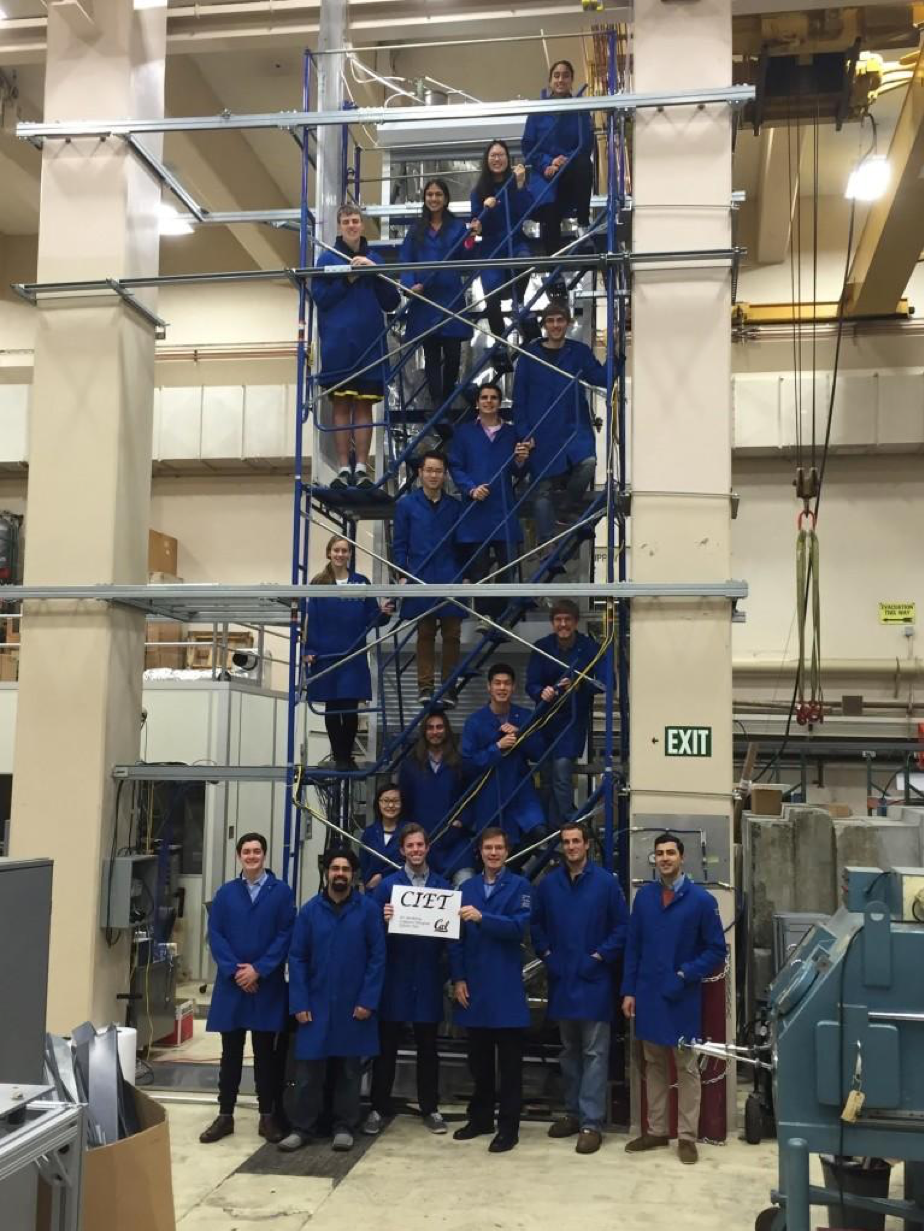
\includegraphics[width=0.8\linewidth]{research_groups/thermal_hydraulics/ciet} \\
		The TH Group in front of CIET. 
	\end{center}
\end{minipage}

\vspace{-0.5cm}
\firststudentrow{
	\studenttile
	{students/clara_alivisatos}
	{Clara Alivisatos}
	{}
	{}
	{Clara, the freshest face in the Thermal Hydraulics Lab and a Berkeley native, got her Bachelor's degree in Physics with a minor in Political Science at Vassar College in New York before heading across the pond to get her Master's degree in Sustainable Energy Futures at Imperial College of London. 
	Her passions include skiing, drinking wine, watching Harry Potter, and traveling.}
}{
	\studenttile
	{students/omar_alzaabi}
	{Omar Alzaabi}
	{}
	{alzaabi@berkeley.edu}
	{Omar is developing methods for quantifying distortions in scaled experiments using frequency response.}
}

\studentrow{
	\studenttile
	{students/shane_gallagher}
	{Shane Gallagher}
	{}
	{shane.gallagher@berkeley.edu}
	{Shane research includes the design and economic feasibility of the power conversion system for fluoride salt cooled high temperature reactors. 
	Shane also enjoys reading, rock climbing, and backpacking.}
}{
	\studenttile
	{students/ishak_johnson}
	{Ishak Johnson}
	{}
	{ishakj5035@berkeley.edu}
	{Ishak, a PhD student from Oklahoma, is developing a set of methods for designing scaled-down experiments for salt-cooled nuclear reactors. 
	Outside the lab, he likes to snowboard, lift, go to the movies, vroom around on his bike, and play video games.}
}

\studentrow{
	\studenttile
	{students/james_kendrick}
	{James Kendrick}
	{}
	{jckendrick@berkeley.edu}
	{James studies the connection between experimental research and commercial regulation, particularly focusing on advanced nuclear reactors. 
	Outside of the lab, he's active in his church community and loves to drink coffee, read, exercise, and bake.}
}{
	\studenttile
	{students/theodore_ong}
	{Theodore Kay Chen Ong}
	{}
	{theodore\_ong@berkeley.edu}
	{Theodore is interested in implementing neutronics effects in thermal hydraulics integral effects tests. 
	He's from Singapore, and he really loves food; he plays bass in church, plays video games and watches dramas.}
}

\studentrow{
	\studenttile
	{students/chris_poresky}
	{Chris Poresky}
	{}
	{chrisporesky@berkeley.edu}
	{Chris works on the design of operator support systems for advanced nuclear reactors by combining interdisciplinary model-based fault detection networks with human-centered design principles. 
	He tries to forget about this at night with a lethal cocktail of writing, jazz, and video games.}
}{}

\grouptitle{Nuclear Physics}

\textbf{Isotope Production:}
The isotopes group has performed a number of cross section measurements to assess the viability of several new isotope production pathways, with emphasis on the production of $^{225}$Ac, $^{64}$Cu, $^{47}$Sc, $^{134}$Ce, $^{86}$Y.  
Measurments take place at both the 88'' cyclotron at LBNL and the high-flux neutron generator (HFNG) located in Etcheverry Hall.  
We collaborate with a number of national labs, where the DOE isotopes program supplies many of the medical isotopes for the U.S.  
Our primary goals are to fill in essential nuclear data gaps, mostly focusing on charged particle and fast-neutron induced reactions, as well as to improve the nuclear modeling of these reactions.  
A better understanding of these reactions will enable the next generation of nuclear medicine, in which ``personalized'' treatments are used to treat cancer.

\textbf{Neutron Scattering:}
Inelastic scattering cross sections have been identified as an important source of uncertainty in neutron transport for current nuclear reactors and for the design of Gen IV reactors. 
Our neutron scattering group is working on the the measurement, modeling and validation of these cross sections. 
This work includes the GENESIS experiment, to measure the energy and angle differential inelastic scattering cross sections for $^{56}$Fe and $^{238}$U. 
Both scattered neutrons and de-excitation gammas will be measured, allowing us to determine both the total inelastic cross section and angular distributions of the outgoing neutrons. 
The uncertainties in both the experiments and the modeling of the cascade of de-excitation gammas are also being characterized, to allow for cross sections to be reported accurately. 
Additionally, work is being done on the ATLAS integral measurement dataset to allow it to be used for validation of reaction calculations.

\textbf{Fission Product Yields:}
The Fast Loading User Facility for Fission Yields (FLUFFY) is a new experimental capability being developed at the 88 inch cyclotron at LBNL.
Once completed, it will feature a pneumatic system that will rapidly transport fissionable samples between a high-flux neutron beam line and an HPGe clover array. 
This will allow for the measurement of independent and cumulative fission yields for products with half-lives down to one second. 
The initial design of FLUFFY is set to be commissioned during an experiment in April 2019. 
Initial measurements using FLUFFY seek to improve fission yield measurements on several short-lived products relevant to the reactor antineutrino anomaly including: $^{92}$Rb, $^{96}$Y, and $^{142}$Cs. 

\firststudentrow{
	\studenttile
	{students/amanda_lewis}
	{Amanda Lewis}
	{}
	{amanda\_lewis@berkeley.edu}
	{Amanda is a fourth year student, working on experimental and modeling uncertainties in nuclear data. 
	Amanda is from upstate New York and enjoys photography, sleeping, and not being sick.}
}{
	\studenttile
	{students/austin_lo}
	{Austin Lo}
	{}
	{loaustin09@berkeley.edu}
	{Austin researches the effects of heavy ion deposition into noble gases and plasmas for potential application to direct energy conversion schemes (e.g. thermionic energy conversion) and advanced nuclear space propulsion systems. 
	Some of his hobbies include specialty coffee, SF excursions, fitness, and motorcycle riding.}
}

\studentrow{
	\studenttile
	{students/eric_matthews}
	{Eric Matthews}
	{}
	{efmatthews@lbl.gov}
	{Eric obtained his high school diploma and AS from the Missouri Academy of Science, Mathematics, and Computing and his B.S. from UC Berkeley. Eric is advised by Dr. Lee Bernstein at LBNL where he intends to perform thesis research on nuclear physics and data related topics. 
	Eric also works with Dr. Bethany Goldblum on the development and application of the Fission Induced Electromagnetic Response (FIER) code, a package for the analytical modeling of delayed gamma-ray spectra.}
}{}

\grouptitle{Dark Matter and Accelerators}

Our group bridges fundamental and applied experimental nuclear physics, utilizing innovative accelerator, ion source, and RF cavity technologies.

One of our primary projects is the Haloscope At Yale Sensitive To Axion Cold dark matter (HAYSTAC). It is a multi-university collaboration searching for axions, a cold dark matter candidate. 
The collaboration consists of UC Berkeley, Yale, and the University of Colorado. 
Housed at Yale, HAYSTAC relies on advanced amplifier, magnet, and cavity technology to achieve extremely low-noise conditions. 
Cooled to hundreds of milliKelvin, the experiment currently operates near the Standard Quantum Limit for noise. 
UC Berkeley’s contribution to the experiment is the microwave cavity. 
The group here focuses on developing high quality factor/high frequency cavities using novel methods like superconducting thin films and Photonic Band Gap structures.

\firststudentrow{
\studenttile
	{students/mauricio_ayllon}
	{Mauricio Ayllon}
	{}
	{mayllon@berkeley.edu}
	{Mauricio works on neutron generators and gamma detection for imaging purposes. In his spare time, he likes traveling and playing sports}
}{
	\studenttile
	{students/al_kenany}
	{Al Kenany}
	{}
	{alkenany@berkeley.edu}
	{Since joining the team, Al has put together a cryostat for testing microwave cavities designed for HAYSTAC. 
	He is currently working on depositing superconducting thin films onto the inner surfaces of cylinders to improve quality factor of the cavities.}
}

\studentrow{
	\studenttile
	{students/sami_lewis}
	{Sami Lewis}
	{}
	{smlewis@berkeley.edu}
	{Sami is a 5th year PhD student working on developing electromagnetic devices for accelerator and dark matter search applications. 
	She enjoys musical theater, cooking, and running.}
}{
	\studenttile
	{students/maria_simanovskaia}
	{Maria Simanovskaia}
	{}
	{simanovskaia@berkeley.edu}
	{Maria's working on designing and testing microwave cavities for the dark matter search HAYSTAC. 
	Originally from St. Petersburg, Russia, she moved to the SF bay area as a child and eventually came to UC Berkeley to study physics and math for undergrad. 
	Now she's enjoying grad school in nuclear engineering. }
}

\grouptitle{Bay Area Neutron Group (BANG)}

The core elements of nuclear physics can be applied to engineer solutions for today’s most pressing nuclear security problems. 
The Bay Area Neutron Group (BANG) combines basic science, algorithm development, radiation detection, and scientific computing to support global nuclear security and nonproliferation. 
BANG brings an end-to-end approach to this area, with research activities spanning basic nuclear physics to the development of advanced detection technologies. 
Current research activities include organic scintillator characterization for fast neutron detection, neutron-induced inelastic scattering reaction cross sections (GENESIS project), neutron spectroscopy using pulse integral spectrum unfolding, and design of compact high-efficiency neutron imagers. 
The group performs experimental physics at a† number of facilities, most notably at the 88-Inch Cyclotron at Lawrence Berkeley National Laboratory. 
To learn more, visit bang.berkeley.edu.

\firststudentrow{
	\studenttile
	{students/christopher_brand}
	{Christopher Brand}
	{}
	{christopher.brand@berkeley.edu}
	{Christopher Brand earned his B.S. in nuclear engineering at UC Berkeley in 2015. He worked as a safety analyst at Lawrence Livermore National Laboratory prior to returning to Berkeley in 2017 to pursue a doctoral degree where his research is focused on neutron imaging and diagnostic systems. }
}{
	\studenttile
	{students/kelly_kmak}
	{Kelly Kmak}
	{}
	{knkmak@berkeley.edu}
	{Kelly is interested in radiochemistry and its practical applications. 
	She has performed research with the UC Berkeley Nuclear Policy Working Group on the thorium fuel cycle and with LLNL on a project to characterize the homologs of element 114 and 115 to predict the properties of these super-heavy elements. 
	She received a B.S. in Chemistry from UC Berkeley in 2016.}
}

\studentrow{
	\studenttile
	{students/adriana_ureche}
	{Adriana Ureche}
	{}
	{adau@berkeley.edu}
	{She earned her B.S. in nuclear engineering at UC Berkeley, where her research focused on low energy nuclear properties and nuclear data. 
	Adriana is interested in fundamental nuclear physics, numerical simulations, and nuclear policy.}
}{}

\restoregeometry
